\secspace
\section{Background: AI Art and Style Mimicry}
\label{sec:motivation}

In this section, we provide critical context in the form of
basic background on current AI art models and style mimicry.

\secspace
\subsection{Text-to-Image Generation}

Since Text-to-image generation was first proposed in
2015~\cite{mansimov2015generating}, a stream of research has proposed newer
model architectures and training methods enabling generation of
higher-quality
images~\cite{radford2015unsupervised,zhang2017stackgan,xu2018attngan,li2019object,zhu2019dm}.  The high level design of
recent models used for AI art
generation~\cite{rombach2022high,ramesh2021zero,d-mini} is shown in
Figure~\ref{fig:diffusion-arch}. During training, the model takes in an image
$x$ and uses a feature extractor $\Phi$ to extract its features, producing
$\Phi(x)$. Simultaneously, a conditional image generator $G$ takes in a
corresponding text caption ($s$) and outputs a predicted feature vector
$G(s)$. Then the parameters of $G$ are optimized so the text feature vector
$G(s)$ matches the image feature vector $\Phi(x)$. At generation time, a user
gives $G$ a text prompt $s_0$, and $G$ outputs an image feature vector
$G(s_0)$. A decoder $D$ then decodes $G(s_0)$ to produce the final generated
image. %Below, we describe $G$, $\Phi$, and $D$ in more detail.

Compared to earlier models based on generative adversarial networks
(GANs) or variational autoencoders
(VAE)~\cite{radford2015unsupervised,zhu2019dm,tao2022df}, more recent
models~\cite{rombach2022high,ramesh2022hierarchical}
leveraging \textit{diffusion} models
produce significantly higher quality images. Feature extractor ($\Phi$) is
used to reduce the dimensionality of the input image to facilitate the
generation process. The extractor $\Phi$ and decoder $D$ are often a pair of
variational autoencoder (VAE)~\cite{rombach2022high,ramesh2021zero}, \ie
extractor (encoder) extracts image features and decoder map features back to
images.

\para{Training Data Sources. } The training datasets of these models
typically contain image/ALT text pairs scraped from the Internet. They
are extremely large, e.g. LAION~\cite{schuhmann2022laion} contains 5 billion
images collected from 3 billion webpages.  

These datasets are subject to minimal curation and governance. Data
collectors typically only filter out data with extremely short or incorrect text captions
(based on an automated text/image alignment metric~\cite{schuhmann2022laion}). % Some
Since copyrighted images are not filtered~\cite{schuhmann2022laion}, these
datasets are rife with private, sensitive content, including copyrighted
artworks.

\secspace
\subsection{Style Mimicry}
\label{sec:mimicry-back}

\begin{figure}[t]
  \centering
  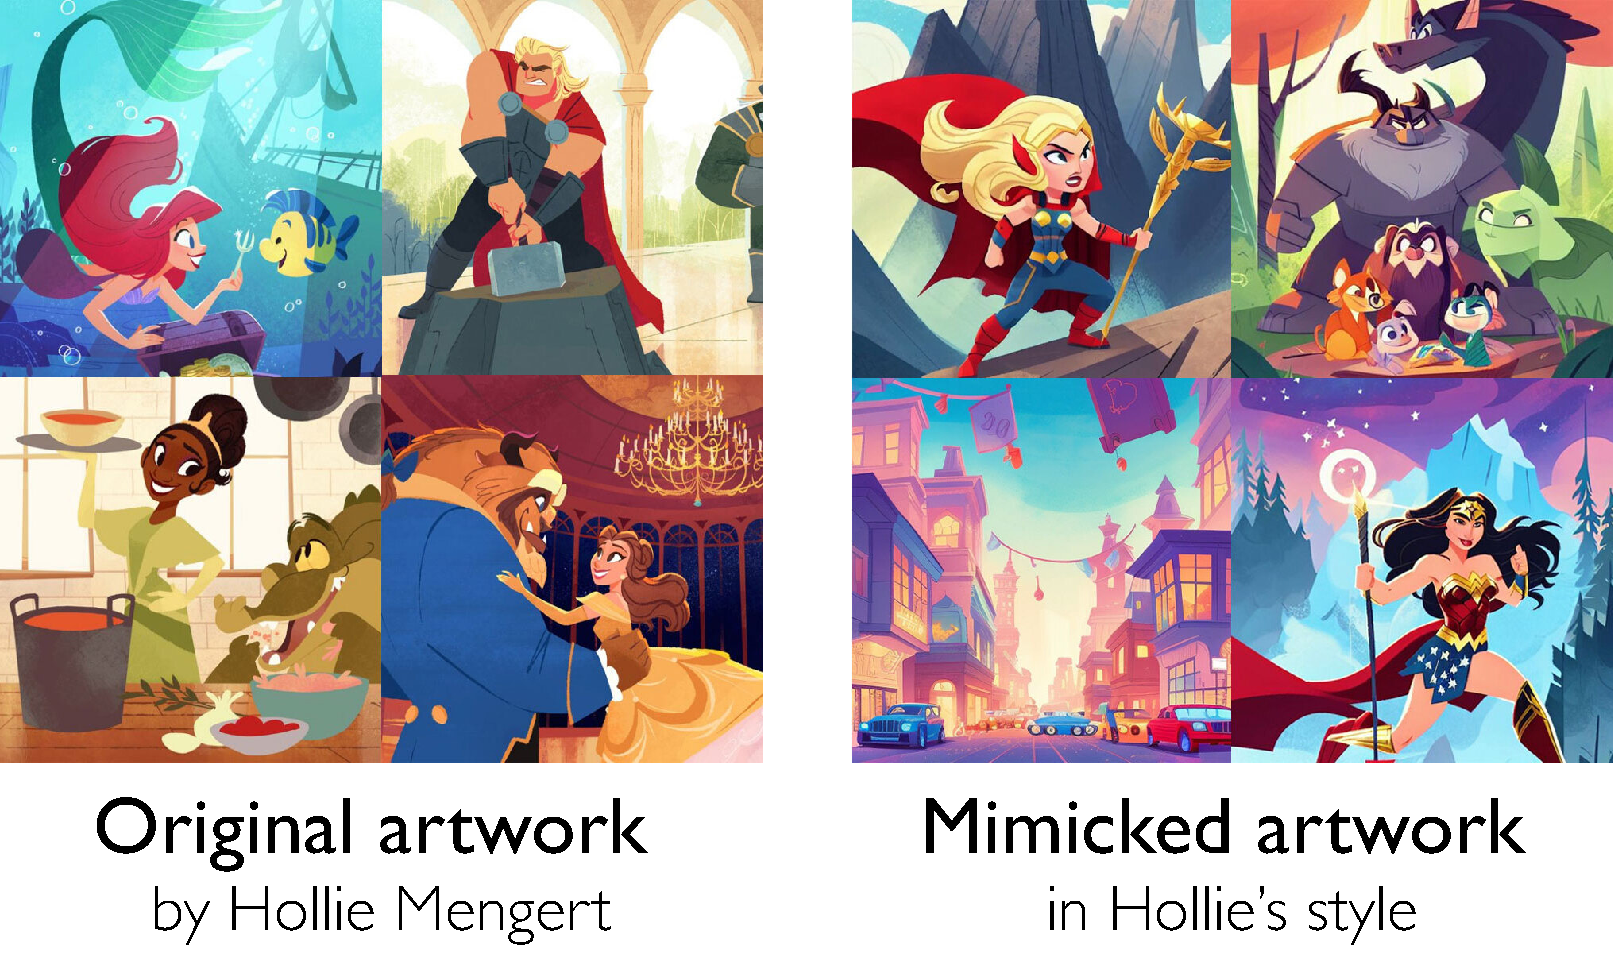
\includegraphics[width=0.95\columnwidth]{plots/overview/hollie-mimic.pdf}
  \vspace{-0.1in}
  \caption{Real-world incident of AI plagiarizing the style of artist Hollie Mengert~\cite{hollie-steal}. {\bf Left}: original artwork by Hollie Mengert. {\bf Right}: plagiarized artwork generated by a model trained to mimic Hollie's style. }
  \label{fig:hollie-mimic}
\end{figure}

In a {\em style mimicry} attack, a bad actor uses an AI art model to create
art in a particular artist's style without their consent. % Style mimicry can
More than 67\% of 
art pieces showcased on a popular AI-art-sharing website leverage style
mimicry~\cite{mid-top-artistname}.

\para{Style mimicry techniques.} Today, a ``mimic'' can easily copy the style of
a victim artist with only an open-source text-to-image model and a few
samples of artwork from the artist. A naive mimicry attack directly queries a
generic text-to-image model using the name of the victim artist. For example,
the prompt ``a painting in the style of Greg Rutkowski'' would cause the
model to generate images in the style of Polish artist Greg Rutkowski. This
is because many of Rutkowski's artworks appear in training datasets of these
generic models labeled with his name.

Naive mimicry can succeed when the artist is well-known and
has a significant amount of art online, but fail on other artists. In more recent
mimicry attacks, a mimic {\em fine-tunes} a
generic text-to-image model on samples of a target artist's work
(as few as $20$ unique pieces) downloaded from online sources. This calibrates the model to
the victim artist's style, identifying important features related to the
victim style and associating these regions in the feature space with the
victim artist's name~\cite{ruiz2022dreambooth,gal2022image}. This enables
style mimicry with impressive accuracy.  The entire fine-tuning process takes
less than 20 minutes on a low-end consumer GPU\footnote{It takes an average
  of 18.3 minutes on a GTX 1080 GPU}.

\para{Real-work mimicry incidents. }
The first well-known incident of mimicry was when a Reddit user stole
American artist Hollie Mengert's style and open-sourced the style-specific
model on Reddit~\cite{hollie-steal}. Figure~\ref{fig:hollie-mimic} has a
side-by-side comparison of Hollie's original artwork and plagiarized artwork
generated via style mimicry. Later, famous cartoonist Sarah Andersen reported
that AI art models can mimic her cartoon drawings~\cite{sarah-andersen}, and
other similar incidents abound~\cite{lensa-steal,sam-steal}.

Several companies~\cite{aigame} have even hosted style mimicry
as a service, allowing users to upload a few art pieces painted by victim
artists and producing new art in the victim styles. CivitAI~\cite{civitai}
built a large online marketplace where people share their customized stable
diffusion models, fine-tuned on certain artwork.  

\begin{figure}[t]
  \centering
  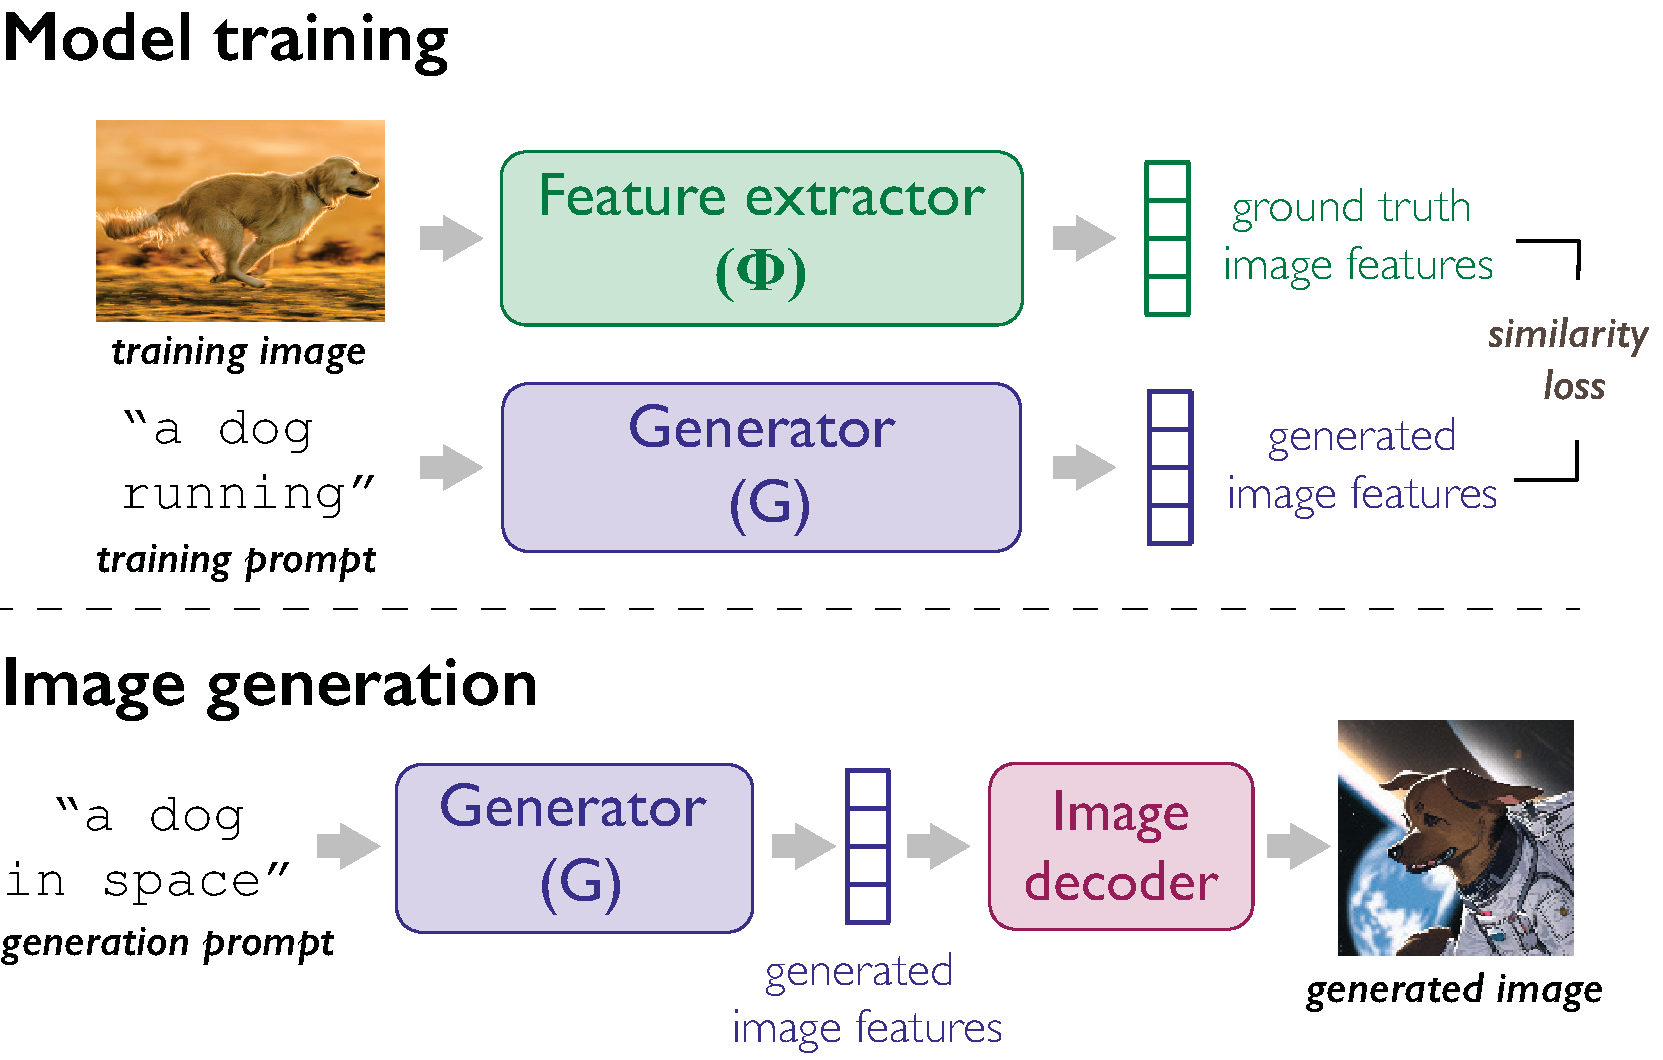
\includegraphics[width=1\columnwidth]{plots/overview/diffusion-arch.pdf}
  \vspace{-0.25in}
  \caption{High level model architecture of text-to-image models. }
  \label{fig:diffusion-arch}
\end{figure}

\secspace
\section{Collaborating with Artists}
\label{sec:artists}
Next, we explain our collaborative relationship with professional artists,
and its significant impact on our key evaluation metrics in this paper. We
also summarize key results from our first user study on views of AI art and
mimicry by members of the artist community.


Artists have spoken out against style mimicry in numerous venues, focusing
particularly on how it violates their intellectual property rights and
threatens their
livelihoods~\cite{guardian-artical,artical-1,artical-2, noai-protest}. Others
have taken direct action. The Concept Art Association raised over \$200K to
fight AI art, and filed a class action lawsuit in the US
against AI art companies~\cite{class-action}. In November 2022, artists
organized a large protest against ArtStation~\cite{noai-protest}, the large
digital art sharing platform that allowed users to post AI artwork without
identification. Anti-AI images flooded the site for several weeks, until
ArtStation banned the protest images~\cite{noai-result}. \revise{Recently, the
Writers Guild of America (WGA) went on strike demanding contractual changes
to ban generative AI~\cite{AIstrike}.}

Members of the professional art community reached out to us in Sept 2022. We
joined online town halls and meetings alongside hundreds of professionals,
including Emmy winners and artists at major film studios. After learning
more, we began an active collaboration with multiple professional artists,
including award-winning artist Karla Ortiz, who leads efforts defending
artists and is lead plaintiff in the class action suit.
The artists helped this project in multiple ways, by 1) sharing experiences
about specific ways AI-art has impacted them and their colleagues; 2) sharing
domain knowledge about what is acceptable to artists in terms of
perturbations on their art; and 3) helping to widely disseminate our user study to
members of their professional organizations, including the Concept Art
Association and the Animation Guild (TAG839).

\para{Evaluation via Direct Feedback from Artists.} Our goal is to help artists
disrupt AI models trying to mimic their artistic style, without adversely
impacting their own artwork. Because ``success'' in this context is highly
subjective (``Did this AI-art successfully mimic Karla's painting style?''),
we believe the only reliable evaluation metric is direct feedback by
professional artists themselves. Therefore, wherever possible, the evaluation
of \system{} is done via detailed user studies engaging members of the
professional artist community, augmented by an empirical score we develop based on
genre prediction using CLIP models.

We deployed two user studies during the course of this project (see
Table~\ref{tab:study-details}). Both are IRB-approved by our institution.  Both
draw participants from professional artists informed via their social circles
and professional networks. The first (Survey 1, \S\ref{sec:user-study},
\S\ref{sec:cloaking-results}), asked participants
about their broad views of AI style mimicry, and then presented them with a
number of inputs and outputs of our tool, and asked them to give ratings
corresponding to key metrics we wanted to evaluate. We select a subset 
of participants from the first study to participate in a 
longer and more in-depth study (Survey 2) where 
they were asked to evaluate the performance of \system{} in 
additional settings (\S\ref{sec:cloaking-results}, \S\ref{sec:robust-eval}, 
\S\ref{sec:counter}, and Appendix~\ref{sec:appendix}). 


\begin{table}[t]
  \centering
  \resizebox{0.49\textwidth}{!}{
  \centering
    \begin{tabular}{ccl}
    \hline
    \textbf{Survey} & \textbf{\begin{tabular}[c]{@{}c@{}} \# of artists\end{tabular}} & \multicolumn{1}{c}{\textbf{Content}} \\ \hline
    Survey 1 & 1156 & \begin{tabular}[c]{@{}l@{}} 1) Broad views of AI art
                        and style mimicry(\S\ref{sec:user-study}) \\
                        2) Glaze's usability, i.e. acceptable levels of cloaking (\S\ref{sec:cloaking-results}) \\
                        3) Glaze performance in disrupting style mimicry (\S\ref{sec:cloaking-results}) \end{tabular} \\ \hline
    
\begin{tabular}[c]{@{}c@{}}
    Survey 2\\(Extension to Survey 1)
    \end{tabular}
    & 151 & \begin{tabular}[c]{@{}l@{}}
    1) Additional performance tests (\S\ref{sec:cloaking-results}) \\
    2) Robustness to advanced scenarios (\S\ref{sec:robust-eval}) \\ and countermeasures (\S\ref{sec:counter}) \\ 
    3) Additional system evaluation (Appendix~\ref{sec:appendix}) \end{tabular} \\ \hline
    \end{tabular}
  }
  \vspace{-0.1in}
  \caption{Information on our user studies: the number of artist participants
    and where we report the results of the studies. We sent Survey 2 to
    some specific participants from survey 1 who volunteered to participate in a
    followup study.}
  \label{tab:study-details}
\end{table}


\secspace
\subsection{Artists' Opinions on Style Mimicry}
\label{sec:user-study}

While we expected artists to view style mimicry negatively, we wanted to
better understand how much individual artists understood this topic and how
many perceived it as a threat. Here we describe results from Survey 1 to
gather perceptions of the potential impact of AI art on existing artists.

\para{Survey Design.} Our survey consisted of both multiple choice and free
response questions to understand how well people understand the concept of AI
art, and how well the models successfully imitate the style of artists.
Additionally, we asked artists about the extent to which they anticipate the
emergence of AI art to impact their artistic activities, such as posting
their art online and their job security.  A handful of professional artists
helped disseminate our survey to their respective artist community groups.
Overall, we collected responses from 1,207 participants, consisting primarily
of professional artists (both full-time (46\%) and part-time/freelancer
(50\%)) and some non-artist members of the art community who felt invested in
the impact of AI art (4\%). Of the participants who consider themselves
artists, their experience varied: <1 year (13\%), 1-5 years (49\%), 5-10
years (19\%), 10+ years (19\%).  Participants' primary art style varied
widely, including: animation, concept art, abstract, anime, game art, digital
2D/3D, illustration, character artwork, storyboarding, traditional
painting/drawing, graphic design, and others.

\para{Key Results.} Our study found that 91\% of the artists have read about
AI art extensively, and either know of or worry about their art being used to
train the models. Artists expect AI mimicry to have a significant impact on artist
community: $97\%$ artists state it will decrease some artists' job security;
$88\%$ artists state it will discourage new students from studying art; and
$70\%$ artists state it will diminish creativity. ``Junior positions will
become extinct,'' as stated by one participant.

Many artists (> 89\% artists) have already or plan to take actions because of
AI mimicry. Over $95\%$ of artists post their artwork online. Out of these
artists, $53\%$ of them anticipate reducing or removing their online artwork,
if they haven't already. Out of these artists, $55\%$ of them believe
reducing their online presence will significantly impact their careers. One
participant stated ``AI art has unmotivated myself from uploading more art
and made me think about all the years I spent learning art.'' $78\%$ of
artists anticipate AI mimicry would impact their job security, and this
percentage increases to $94\%$ for the job security of newer
artists. Further, $24\%$ of artists believe AI art has \textit{already}
impacted their job security, and an additional $53\%$ expect to be affected
within the next 3 years. Over $51\%$ of artists expressed interest in
proactive measures, such as personally joining class action lawsuits against
AI companies.  

Professional artists thought AI mimicry was very successful at mimicking the
style of specific artists.  We showed the artists examples of original
artwork from $23$ artists, and the artwork generated by a model
attempting to mimic their styles (detailed mimicry setup in
\S\ref{sec:eval-cloak}).  $77\%$ of artists found the AI model
\textit{successfully} or \textit{very successfully} mimic the styles of
victim artists, with one stating ``it's shocking how well AI can mimic the
original artwork.''  Additionally, $19\%$ of participants thought the AI
mimicry is somewhat successful, leaving only $< 5\%$ of artists rating the
mimicry as unsuccessful.  Several artists also pointed out that, as artists,
upon close inspection they could spot differences between the AI art and
originals, but were skeptical the general public would notice them.
%the same disparities.

A significant concern of most participants, surprisingly, is not just the
existence of AI art, but rather scraping of existing artworks without
permission or compensation.  As one participant stated: ``If artists are paid
to have their pieces be used and asked permission, and if people had to pay
to use that AI software with those pieces in it, I would have no problem.''
However, without consent to use their artwork to train the models, ``it's
incredibly disrespectful to the artist to have their work `eaten' by a
machine [after] many years to grow our skills and develop our styles.''